\documentclass[aspectratio=169]{beamer}
\usepackage[utf8]{inputenc}
\usepackage[T1]{fontenc}
\usepackage{amsmath,amssymb}
\usepackage{graphicx}
\usepackage{booktabs}
\usepackage{listings}
\usepackage{tikz}
\usetikzlibrary{shapes,arrows,positioning}

\usetheme{Madrid}
\usecolortheme{whale}
\setbeamertemplate{blocks}[rounded][shadow=false]

\definecolor{codegreen}{rgb}{0,0.5,0}
\definecolor{codegray}{rgb}{0.5,0.5,0.5}
\definecolor{codepurple}{rgb}{0.58,0,0.82}
\definecolor{backcolour}{rgb}{0.95,0.95,0.97}

\lstset{
  backgroundcolor=\color{backcolour},
  basicstyle=\ttfamily\tiny,
  keywordstyle=\color{blue!80!black}\bfseries,
  commentstyle=\color{codegreen}\itshape,
  stringstyle=\color{codepurple},
  breaklines=true,
  frame=none,
  numbers=left,
  numberstyle=\tiny\color{codegray},
  tabsize=2
}

\title[Deep RL for Robotics]{Deep Reinforcement Learning\\for Autonomous Robot Navigation}
\subtitle{From Simulation to Real-World Deployment}
\author[Chen \& Nakamura]{Dr.\ Wei Chen\inst{1} \and Prof.\ Yuki Nakamura\inst{2}}
\institute[MIT \& UTokyo]{\inst{1}MIT CSAIL \and \inst{2}University of Tokyo}
\date[ICRA 2025]{International Conference on Robotics and Automation\\May 2025}

\begin{document}

% ──── Title Slide ────
\begin{frame}
  \titlepage
\end{frame}

% ──── Outline ────
\begin{frame}{Outline}
  \tableofcontents
\end{frame}

% ════════════════════════════════
\section{Introduction}
% ════════════════════════════════

\begin{frame}{The Challenge of Autonomous Navigation}
  \begin{columns}[T]
    \begin{column}{0.55\textwidth}
      \textbf{Key challenges:}
      \begin{itemize}
        \item Complex, dynamic environments
        \item Partial observability from onboard sensors
        \item Real-time decision making under uncertainty
        \item Safe exploration during training
        \item Sim-to-real transfer gap
      \end{itemize}

      \vspace{0.5cm}
      \textbf{Our approach:}\\
      Use deep reinforcement learning with domain randomization and curriculum learning to train navigation policies in simulation, then transfer to real robots.
    \end{column}
    \begin{column}{0.4\textwidth}
      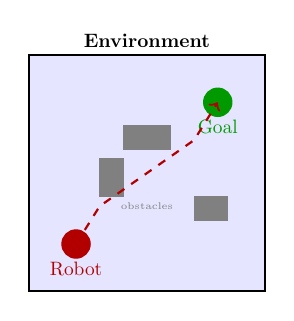
\begin{tikzpicture}[scale=0.6, every node/.style={scale=0.7}]
        \draw[thick, fill=blue!10] (0,0) rectangle (5,5);
        \node at (2.5,5.3) {\textbf{Environment}};
        \filldraw[red!70!black] (1,1) circle (0.3) node[below=4pt] {Robot};
        \filldraw[green!60!black] (4,4) circle (0.3) node[below=4pt] {Goal};
        \filldraw[gray] (2,3) rectangle (3,3.5);
        \filldraw[gray] (1.5,2) rectangle (2,2.8);
        \filldraw[gray] (3.5,1.5) rectangle (4.2,2);
        \node[gray] at (2.5,1.8) {\tiny obstacles};
        \draw[->,thick,red!70!black,dashed] (1,1) -- (1.5,1.8) -- (2.5,2.5) -- (3.5,3.2) -- (4,4);
      \end{tikzpicture}
    \end{column}
  \end{columns}
\end{frame}

% ════════════════════════════════
\section{Background}
% ════════════════════════════════

\begin{frame}{Reinforcement Learning Basics}
  \begin{block}{Markov Decision Process (MDP)}
    An MDP is defined by the tuple $(\mathcal{S}, \mathcal{A}, P, R, \gamma)$:
    \begin{itemize}
      \item $\mathcal{S}$: state space \quad $\mathcal{A}$: action space
      \item $P(s' | s, a)$: transition dynamics
      \item $R(s, a)$: reward function \quad $\gamma$: discount factor
    \end{itemize}
  \end{block}

  \vspace{0.3cm}
  \begin{alertblock}{Objective}
    Find policy $\pi^*$ that maximizes expected cumulative reward:
    \begin{equation*}
      \pi^* = \arg\max_\pi \; \mathbb{E}_{\tau \sim \pi} \left[ \sum_{t=0}^{T} \gamma^t R(s_t, a_t) \right]
    \end{equation*}
  \end{alertblock}

  \begin{exampleblock}{Key Insight}
    Deep RL uses neural networks to approximate $\pi(a|s)$ or $Q(s,a)$, enabling learning in continuous, high-dimensional state-action spaces.
  \end{exampleblock}
\end{frame}

\begin{frame}{Policy Gradient Methods}
  \textbf{Proximal Policy Optimization (PPO)} is our algorithm of choice:

  \begin{equation*}
    L^{\text{CLIP}}(\theta) = \hat{\mathbb{E}}_t \left[ \min\left( r_t(\theta) \hat{A}_t, \; \text{clip}(r_t(\theta), 1{-}\epsilon, 1{+}\epsilon) \hat{A}_t \right) \right]
  \end{equation*}

  where $r_t(\theta) = \frac{\pi_\theta(a_t|s_t)}{\pi_{\theta_{\text{old}}}(a_t|s_t)}$ is the probability ratio.

  \vspace{0.3cm}
  \textbf{Advantages of PPO:}
  \begin{enumerate}
    \item Stable training with clipped objective
    \item Sample efficient with multiple epochs per batch
    \item Works well with both continuous and discrete actions
    \item Easy to parallelize across environments
  \end{enumerate}
\end{frame}

% ════════════════════════════════
\section{Methodology}
% ════════════════════════════════

\begin{frame}{System Architecture}
  \begin{center}
  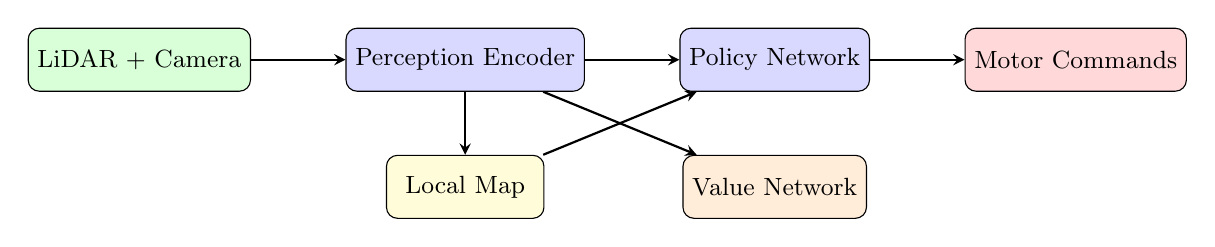
\begin{tikzpicture}[
    node distance=1.2cm,
    box/.style={rectangle, draw, fill=blue!15, rounded corners, minimum width=2cm, minimum height=0.8cm, font=\small},
    arrow/.style={->, thick, >=stealth}
  ]
    \node[box, fill=green!15] (sensor) {LiDAR + Camera};
    \node[box, right=of sensor] (encoder) {Perception Encoder};
    \node[box, right=of encoder] (policy) {Policy Network};
    \node[box, right=of policy, fill=red!15] (action) {Motor Commands};

    \node[box, below=0.8cm of encoder, fill=yellow!15] (map) {Local Map};
    \node[box, below=0.8cm of policy, fill=orange!15] (value) {Value Network};

    \draw[arrow] (sensor) -- (encoder);
    \draw[arrow] (encoder) -- (policy);
    \draw[arrow] (policy) -- (action);
    \draw[arrow] (encoder) -- (map);
    \draw[arrow] (map) -- (policy);
    \draw[arrow] (encoder) -- (value);
  \end{tikzpicture}
  \end{center}

  \vspace{0.3cm}
  \begin{itemize}
    \item \textbf{Perception Encoder}: CNN processes LiDAR scans and depth images
    \item \textbf{Local Map}: Occupancy grid built from sensor history
    \item \textbf{Policy Network}: Outputs velocity commands $(v, \omega)$
    \item \textbf{Value Network}: Estimates state value for advantage computation
  \end{itemize}
\end{frame}

\begin{frame}[fragile]{Training Code}
  \begin{lstlisting}[language=Python]
import torch
from stable_baselines3 import PPO
from navigation_env import NavigationEnv

# Create vectorized training environments
env = make_vec_env(NavigationEnv, n_envs=16, env_kwargs={
    "map_size": 10.0,
    "max_obstacles": 20,
    "domain_randomization": True,
})

# Configure PPO with custom network
model = PPO(
    "MultiInputPolicy",
    env,
    learning_rate=3e-4,
    n_steps=2048,
    batch_size=256,
    n_epochs=10,
    gamma=0.99,
    gae_lambda=0.95,
    clip_range=0.2,
    verbose=1,
    tensorboard_log="./logs/",
)

# Train for 10M timesteps with curriculum
model.learn(total_timesteps=10_000_000,
            callback=CurriculumCallback())
  \end{lstlisting}
\end{frame}

% ════════════════════════════════
\section{Results}
% ════════════════════════════════

\begin{frame}{Simulation Results}
  \begin{table}
    \centering
    \caption{Navigation performance across environment difficulties}
    \begin{tabular}{@{}lccc@{}}
      \toprule
      \textbf{Method} & \textbf{Success (\%)} & \textbf{Collision (\%)} & \textbf{Avg.\ Time (s)} \\
      \midrule
      Bug2 Algorithm       & 62.3 & 15.2 & 34.7 \\
      RRT*                 & 78.1 & 8.4  & 28.3 \\
      DWA Planner          & 71.5 & 12.1 & 31.2 \\
      Vanilla PPO          & 81.4 & 6.7  & 22.8 \\
      SAC                  & 83.2 & 5.9  & 21.5 \\
      \midrule
      \textbf{Ours (PPO+DR+CL)} & \textbf{94.7} & \textbf{2.1} & \textbf{18.3} \\
      \bottomrule
    \end{tabular}
  \end{table}

  \begin{itemize}
    \item DR = Domain Randomization, CL = Curriculum Learning
    \item Evaluated on 1000 randomly generated environments
    \item Our method achieves \textbf{94.7\%} success rate with only \textbf{2.1\%} collisions
  \end{itemize}
\end{frame}

\begin{frame}{Sim-to-Real Transfer}
  \begin{columns}[T]
    \begin{column}{0.5\textwidth}
      \textbf{Real-world experiments:}
      \begin{itemize}
        \item TurtleBot3 Waffle Pi platform
        \item Hokuyo LiDAR + Intel RealSense
        \item 5 different indoor environments
        \item 50 trials per environment
      \end{itemize}

      \vspace{0.3cm}
      \textbf{Key findings:}
      \begin{enumerate}
        \item Zero-shot transfer: 78\% success
        \item With 100 real episodes fine-tuning: 91\% success
        \item Average planning time: 12ms (real-time)
      \end{enumerate}
    \end{column}
    \begin{column}{0.45\textwidth}
      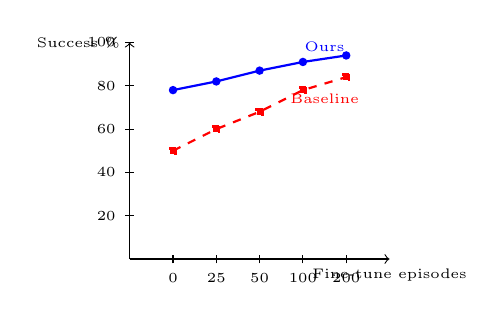
\begin{tikzpicture}[scale=0.55]
        \begin{scope}
          \draw[->] (0,0) -- (6,0) node[below] {\tiny Fine-tune episodes};
          \draw[->] (0,0) -- (0,5) node[left] {\tiny Success \%};
          \foreach \y in {20,40,60,80,100} {
            \draw (-0.1,{\y/20}) -- (0.1,{\y/20});
            \node[left,font=\tiny] at (-0.1,{\y/20}) {\y};
          }
          \foreach \x/\l in {1/0,2/25,3/50,4/100,5/200} {
            \draw (\x,-0.1) -- (\x,0.1);
            \node[below,font=\tiny] at (\x,-0.1) {\l};
          }
          \draw[thick,blue,mark=*] plot coordinates {(1,3.9) (2,4.1) (3,4.35) (4,4.55) (5,4.7)};
          \draw[thick,red,dashed,mark=square*] plot coordinates {(1,2.5) (2,3.0) (3,3.4) (4,3.9) (5,4.2)};
          \node[font=\tiny,blue] at (4.5,4.9) {Ours};
          \node[font=\tiny,red] at (4.5,3.7) {Baseline};
        \end{scope}
      \end{tikzpicture}
    \end{column}
  \end{columns}
\end{frame}

% ════════════════════════════════
\section{Conclusion}
% ════════════════════════════════

\begin{frame}{Summary and Future Work}
  \textbf{Key contributions:}
  \begin{enumerate}
    \item Novel deep RL framework for autonomous navigation combining PPO with domain randomization and curriculum learning
    \item State-of-the-art simulation performance: \textbf{94.7\%} success rate
    \item Successful sim-to-real transfer with \textbf{91\%} real-world success after minimal fine-tuning
    \item Real-time inference at \textbf{12ms} per decision on embedded hardware
  \end{enumerate}

  \vspace{0.5cm}
  \textbf{Future directions:}
  \begin{itemize}
    \item Multi-robot coordination and formation control
    \item Outdoor navigation with GPS-denied environments
    \item Integration with semantic scene understanding
    \item Formal safety guarantees via constrained RL
  \end{itemize}

  \vspace{0.5cm}
  \centering
  \textbf{\large Thank you! Questions?}\\[0.3cm]
  \small\texttt{weichen@mit.edu} \quad|\quad \texttt{github.com/wchen/nav-rl}
\end{frame}

% ──── References ────
\begin{frame}[allowframebreaks]{References}
  \tiny
  \begin{thebibliography}{10}
  \bibitem{schulman2017ppo} J.~Schulman et al., ``Proximal policy optimization algorithms,'' \textit{arXiv:1707.06347}, 2017.
  \bibitem{tobin2017domain} J.~Tobin et al., ``Domain randomization for transferring deep neural networks from simulation to the real world,'' in \textit{IROS}, 2017.
  \bibitem{mnih2015dqn} V.~Mnih et al., ``Human-level control through deep reinforcement learning,'' \textit{Nature}, vol.~518, pp.~529--533, 2015.
  \bibitem{tai2017virtual} L.~Tai, G.~Paolo, and M.~Liu, ``Virtual-to-real deep reinforcement learning: Continuous control of mobile robots for mapless navigation,'' in \textit{IROS}, 2017.
  \end{thebibliography}
\end{frame}

\end{document}
